% Full_diagram.tex — Publication-ready TikZ: First Proof workflow
\documentclass[border=10pt]{standalone}
\usepackage[T1]{fontenc}
\usepackage{lmodern}
\usepackage{tikz}
\usetikzlibrary{positioning,arrows.meta,fit,backgrounds,calc}

% ── Colours ─────────────────────────────────────────────────────────
\definecolor{agenticBg}{RGB}{218,232,252}
\definecolor{webBg}{RGB}{255,243,205}
\definecolor{leanBg}{RGB}{215,238,215}
\definecolor{nodeBlue}{RGB}{184,212,240}
\definecolor{nodeGreen}{RGB}{200,235,200}
\definecolor{nodeGray}{RGB}{230,230,230}
\definecolor{arrowCol}{RGB}{60,60,60}
\definecolor{borderCol}{RGB}{100,100,100}
\definecolor{dBlue}{RGB}{100,130,180}
\definecolor{dAmber}{RGB}{180,140,50}
\definecolor{dGreen}{RGB}{80,140,80}
\definecolor{hdrCol}{RGB}{50,50,50}

% ── Styles ──────────────────────────────────────────────────────────
\tikzset{
  proc/.style={rectangle,rounded corners=4pt,draw=borderCol,
    line width=0.6pt,fill=nodeGray,minimum width=30mm,
    minimum height=9mm,font=\sffamily\small,align=center,inner sep=4pt},
  ai/.style={proc,fill=nodeBlue},
  doc/.style={proc,fill=nodeGreen,minimum width=32mm},
  annot/.style={font=\sffamily\scriptsize\itshape,text=gray!55!black,
    inner sep=1pt,align=center},
  lbl/.style={font=\sffamily\scriptsize,text=black!60,inner sep=1pt,
    align=center},
  sechdr/.style={font=\sffamily\large\bfseries},
  arr/.style={-{Stealth[length=5pt,width=3.5pt]},line width=0.6pt,
    color=arrowCol},
  biarr/.style={{Stealth[length=5pt,width=3.5pt]}-{Stealth[length=5pt,
    width=3.5pt]},line width=0.6pt,color=arrowCol},
  reg/.style={rounded corners=8pt,line width=1.1pt,dashed,inner sep=14pt},
}

\begin{document}
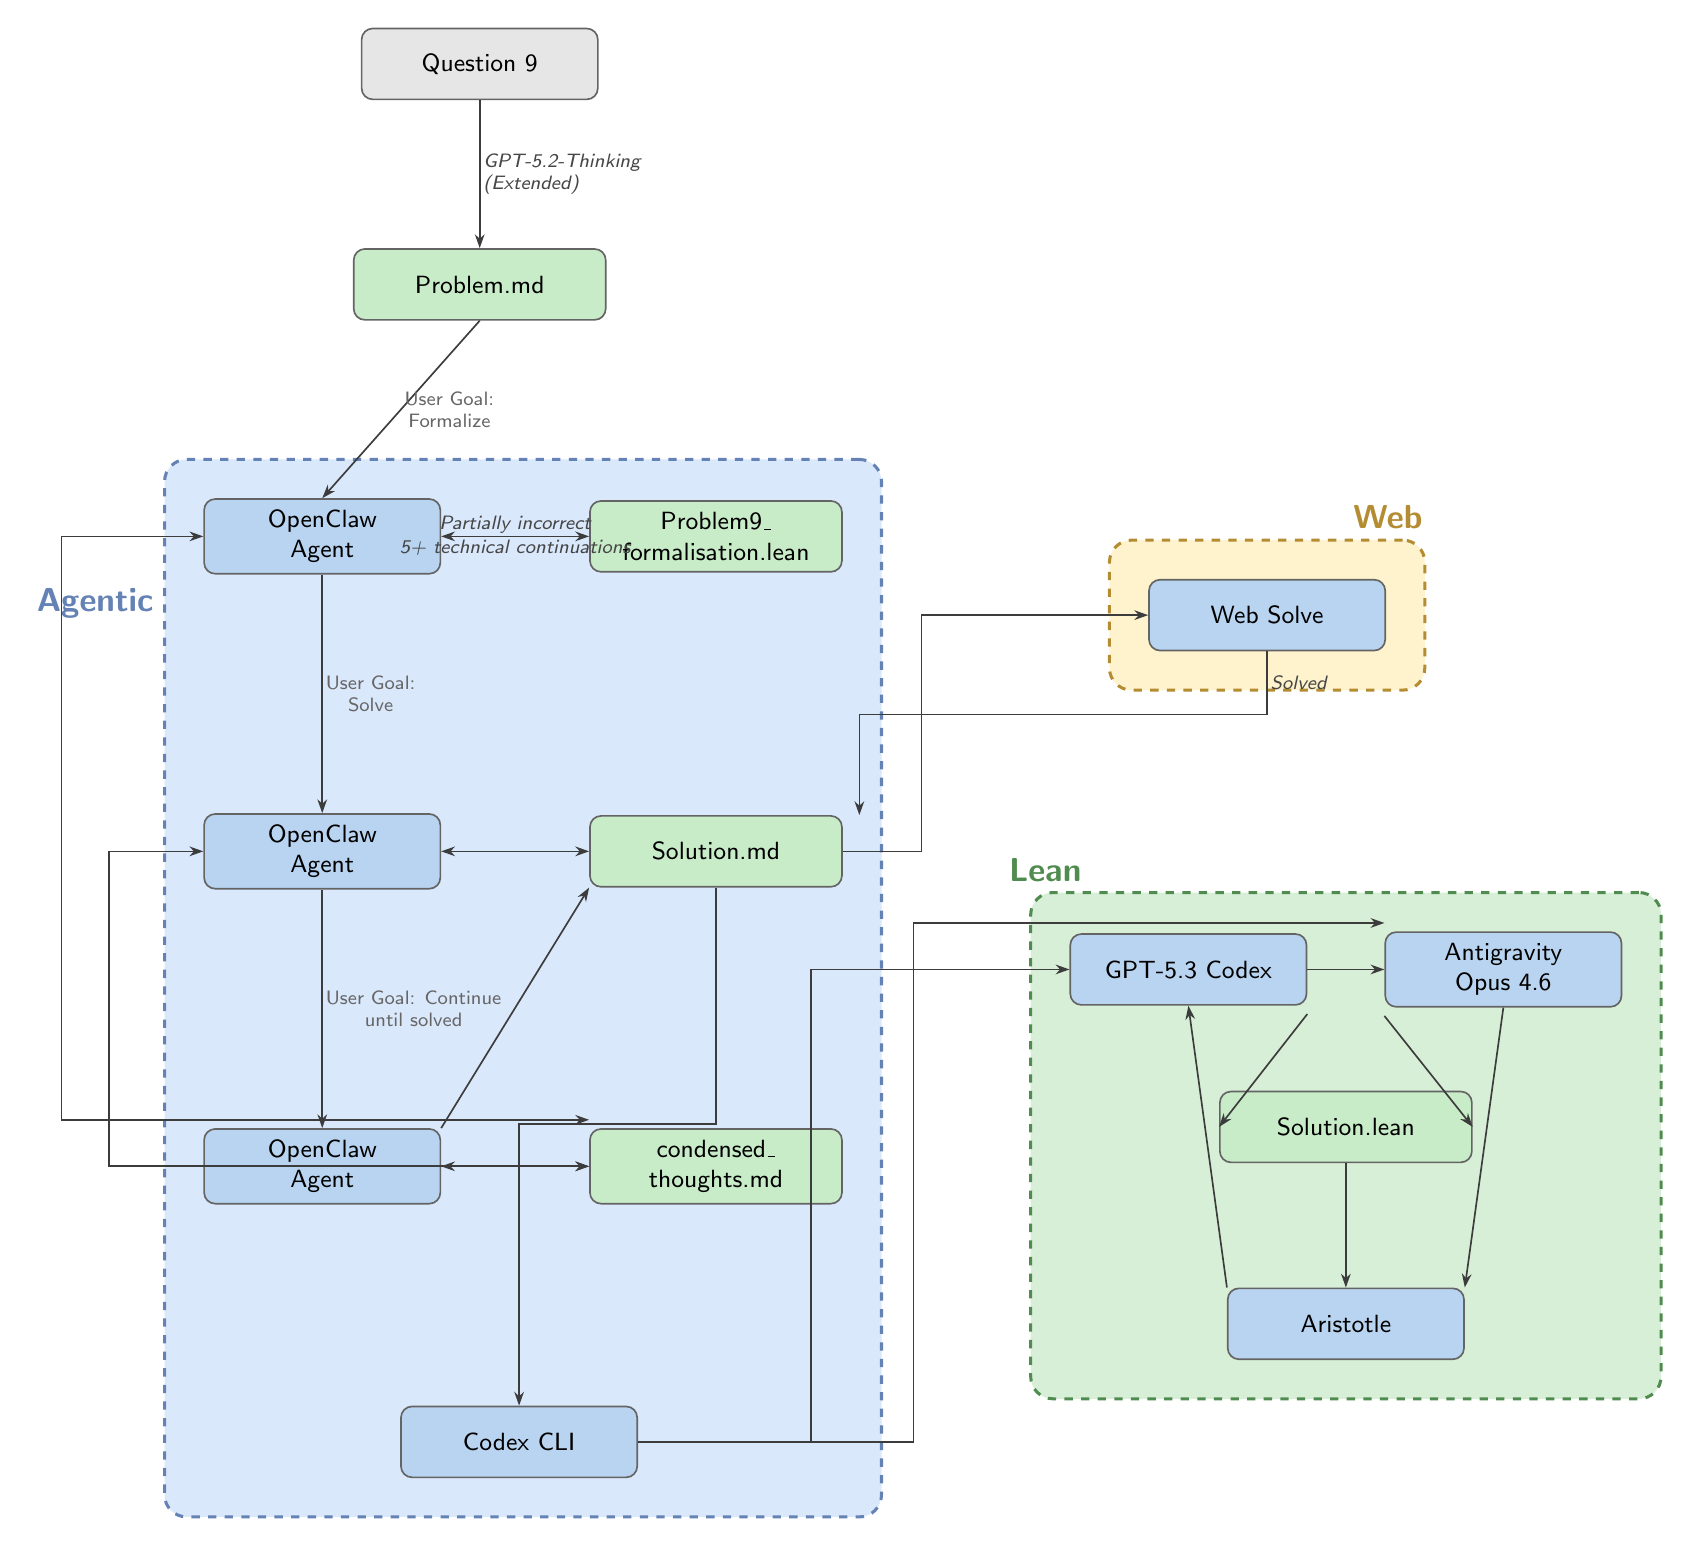
\begin{tikzpicture}

% =====================================================================
%  TOP — Question 9 → Problem.md  (single arrow with GPT label)
% =====================================================================
\node[proc] (q9) at (-3,0) {Question 9};
\node[doc]  (pmd) at (-3,-2.8) {Problem.md};
\draw[arr] (q9) -- node[annot,right,align=left]
  {GPT-5.2-Thinking\\(Extended)} (pmd);

% =====================================================================
%  AGENTIC — Agents on left, docs in middle, Codex CLI at bottom
% =====================================================================

% --- Agents (left column) ---
\node[ai] (oc1) at (-5,-6)    {OpenClaw\\Agent};
\node[ai] (oc2) at (-5,-10)   {OpenClaw\\Agent};
\node[ai] (oc3) at (-5,-14)   {OpenClaw\\Agent};

% --- Middle docs (right of agents) ---
\node[doc] (p9l) at (0,-6)    {Problem9\_\\formalisation.lean};
\node[doc] (smd) at (0,-10)   {Solution.md};
\node[doc] (ctm) at (0,-14)   {condensed\_\\thoughts.md};

% --- Codex CLI ---
\node[ai] (ccli) at (-2.5,-17.5) {Codex CLI};

% ----- Arrows inside Agentic -----

% Problem.md → OC1 with "User Goal: Formalize"
\draw[arr] (pmd.south) -- node[lbl,right] {User Goal:\\Formalize} (oc1.north);

% OC1 ↔ P9_formalisation.lean
\draw[biarr] (oc1) --
  node[annot,above] {Partially incorrect}
  node[annot,below] {5+ technical continuations}
  (p9l);

% OC1 → OC2 with "User Goal: Solve"
\draw[arr] (oc1) -- node[lbl,right] {User Goal:\\Solve} (oc2);

% OC2 ↔ Solution.md
\draw[biarr] (oc2) -- (smd);

% OC2 → OC3 with "User Goal: Continue until solved"
\draw[arr] (oc2) -- node[lbl,right] {User Goal: Continue\\until solved} (oc3);

% OC3 → Solution.md (diagonal upward)
\draw[arr] (oc3.north east) -- (smd.south west);

% All three agents ↔ condensed_thoughts.md
% Route left, then down along a vertical bus, then right to ctm.
\draw[biarr] (oc1.west) -- ++(-1.8,0) |- ([yshift=3pt]ctm.north west);
\draw[biarr] (oc2.west) -- ++(-1.2,0) |- (ctm.west);
\draw[biarr] (oc3) -- (ctm);

% Solution.md → Codex CLI
\draw[arr] (smd.south) -- ++(0,-3) -| (ccli.north);

% =====================================================================
%  WEB — positioned to the RIGHT, above Lean
% =====================================================================
\node[ai] (ws) at (7,-7) {Web Solve};

% Solution.md → Web Solve (rightward then up)
\draw[arr] (smd.east) -- ++(1,0) |- (ws.west);

% Web Solve → Solution.md (labeled "Solved")
\draw[arr] (ws.south) -- ++(0,-0.8)
  node[annot,right,pos=0.5] {Solved}
  -| ([xshift=6pt]smd.north east);

% =====================================================================
%  LEAN — just below Web, on the RIGHT side
%  Ring: GPT-5.3 → Antigravity → Aristotle → GPT-5.3
%  Solution.lean in the centre
% =====================================================================
\node[ai]  (g53) at (6,-11.5)  {GPT-5.3 Codex};
\node[ai]  (ag)  at (10,-11.5)  {Antigravity\\Opus 4.6};
\node[ai]  (ari) at (8,-16)    {Aristotle};
\node[doc] (sl)  at (8,-13.5)  {Solution.lean};

% Ring arrows (one-directional cycle, with bends to avoid overlap)
\draw[arr] (g53.east) -- (ag.west);
\draw[arr] (ag.south) -- (ari.north east);
\draw[arr] (ari.north west) -- (g53.south);

% Ring nodes → Solution.lean (centre — use distinct anchors)
\draw[arr] ([yshift=-3pt]g53.south east) -- (sl.west);
\draw[arr] ([yshift=-3pt]ag.south west)  -- (sl.east);
\draw[arr] (sl.south) -- (ari.north);

% Codex CLI → GPT-5.3 and Antigravity (rightward routes)
\draw[arr] (ccli.east) -- ++(2.2,0) |- (g53.west);
\draw[arr] (ccli.east) -- ++(3.5,0) |- ([yshift=3pt]ag.north west);

% =====================================================================
%  BACKGROUND REGIONS
% =====================================================================
\begin{scope}[on background layer]
  % Agentic (blue) — left side
  \node[reg,draw=dBlue,fill=agenticBg,
    fit=(oc1)(oc2)(oc3)(p9l)(smd)(ctm)(ccli),
    label={[sechdr,text=dBlue]above left:Agentic}
  ] (abox) {};

  % Web (amber/yellow) — upper right
  \node[reg,draw=dAmber,fill=webBg,
    fit=(ws),
    label={[sechdr,text=dAmber]above right:Web}
  ] (wbox) {};

  % Lean (green) — below Web, on the right
  \node[reg,draw=dGreen,fill=leanBg,
    fit=(g53)(ag)(sl)(ari),
    label={[sechdr,text=dGreen]above left:Lean}
  ] (lbox) {};
\end{scope}

\end{tikzpicture}
\end{document}
